\documentclass[a4paper]{article}\usepackage[]{graphicx}\usepackage[]{color}
%% maxwidth is the original width if it is less than linewidth
%% otherwise use linewidth (to make sure the graphics do not exceed the margin)
\makeatletter
\def\maxwidth{ %
  \ifdim\Gin@nat@width>\linewidth
    \linewidth
  \else
    \Gin@nat@width
  \fi
}
\makeatother

\definecolor{fgcolor}{rgb}{0.345, 0.345, 0.345}
\newcommand{\hlnum}[1]{\textcolor[rgb]{0.686,0.059,0.569}{#1}}%
\newcommand{\hlstr}[1]{\textcolor[rgb]{0.192,0.494,0.8}{#1}}%
\newcommand{\hlcom}[1]{\textcolor[rgb]{0.678,0.584,0.686}{\textit{#1}}}%
\newcommand{\hlopt}[1]{\textcolor[rgb]{0,0,0}{#1}}%
\newcommand{\hlstd}[1]{\textcolor[rgb]{0.345,0.345,0.345}{#1}}%
\newcommand{\hlkwa}[1]{\textcolor[rgb]{0.161,0.373,0.58}{\textbf{#1}}}%
\newcommand{\hlkwb}[1]{\textcolor[rgb]{0.69,0.353,0.396}{#1}}%
\newcommand{\hlkwc}[1]{\textcolor[rgb]{0.333,0.667,0.333}{#1}}%
\newcommand{\hlkwd}[1]{\textcolor[rgb]{0.737,0.353,0.396}{\textbf{#1}}}%

\usepackage{framed}
\makeatletter
\newenvironment{kframe}{%
 \def\at@end@of@kframe{}%
 \ifinner\ifhmode%
  \def\at@end@of@kframe{\end{minipage}}%
  \begin{minipage}{\columnwidth}%
 \fi\fi%
 \def\FrameCommand##1{\hskip\@totalleftmargin \hskip-\fboxsep
 \colorbox{shadecolor}{##1}\hskip-\fboxsep
     % There is no \\@totalrightmargin, so:
     \hskip-\linewidth \hskip-\@totalleftmargin \hskip\columnwidth}%
 \MakeFramed {\advance\hsize-\width
   \@totalleftmargin\z@ \linewidth\hsize
   \@setminipage}}%
 {\par\unskip\endMakeFramed%
 \at@end@of@kframe}
\makeatother

\definecolor{shadecolor}{rgb}{.97, .97, .97}
\definecolor{messagecolor}{rgb}{0, 0, 0}
\definecolor{warningcolor}{rgb}{1, 0, 1}
\definecolor{errorcolor}{rgb}{1, 0, 0}
\newenvironment{knitrout}{}{} % an empty environment to be redefined in TeX

\usepackage{alltt}
\usepackage{geometry}
\usepackage{placeins}
\IfFileExists{upquote.sty}{\usepackage{upquote}}{}
\begin{document}




\begin{knitrout}
\definecolor{shadecolor}{rgb}{0.969, 0.969, 0.969}\color{fgcolor}\begin{kframe}
\begin{alltt}
\hlcom{# .define.fonts <- function () \{}
\hlcom{#     quartzFonts(avenir =    c('Avenir Book', 'Avenir Black', 'Avenir Book Oblique', 'Avenir Black Oblique'),}
\hlcom{#                 helvetica = c('Helvetica New Light', 'Helvetica New Bold', 'Helvetica New Light Italic', 'Helvetica New Bold Italic'),}
\hlcom{#                 cmodern = c('CMU Serif', 'CMU Serif Extra','CMU Classical Serif','CMU Serif Extra'))}
\hlcom{# \}}
\hlcom{# .define.fonts()}
\end{alltt}
\end{kframe}
\end{knitrout}

\begin{knitrout}
\definecolor{shadecolor}{rgb}{0.969, 0.969, 0.969}\color{fgcolor}\begin{kframe}
\begin{alltt}
\hlkwd{library}\hlstd{(extrafont)}
\end{alltt}


{\ttfamily\noindent\itshape\color{messagecolor}{\#\# Registering fonts with R}}\begin{alltt}
\hlkwd{loadfonts}\hlstd{()}
\end{alltt}


{\ttfamily\noindent\itshape\color{messagecolor}{\#\# .Keyboard already registered with pdfFonts().}}

{\ttfamily\noindent\itshape\color{messagecolor}{\#\# Andale Mono already registered with pdfFonts().}}

{\ttfamily\noindent\itshape\color{messagecolor}{\#\# More than one version of regular/bold/italic found for Apple Braille. Skipping setup for this font.}}

{\ttfamily\noindent\itshape\color{messagecolor}{\#\# AppleMyungjo already registered with pdfFonts().}}

{\ttfamily\noindent\itshape\color{messagecolor}{\#\# Arial Black already registered with pdfFonts().}}

{\ttfamily\noindent\itshape\color{messagecolor}{\#\# Arial already registered with pdfFonts().}}

{\ttfamily\noindent\itshape\color{messagecolor}{\#\# Arial Narrow already registered with pdfFonts().}}

{\ttfamily\noindent\itshape\color{messagecolor}{\#\# Arial Rounded MT Bold already registered with pdfFonts().}}

{\ttfamily\noindent\itshape\color{messagecolor}{\#\# Arial Unicode MS already registered with pdfFonts().}}

{\ttfamily\noindent\itshape\color{messagecolor}{\#\# Bodoni Ornaments already registered with pdfFonts().}}

{\ttfamily\noindent\itshape\color{messagecolor}{\#\# Bodoni 72 Smallcaps already registered with pdfFonts().}}

{\ttfamily\noindent\itshape\color{messagecolor}{\#\# No regular (non-bold, non-italic) version of . Skipping setup for this font.}}

{\ttfamily\noindent\itshape\color{messagecolor}{\#\# No regular (non-bold, non-italic) version of Brush Script MT. Skipping setup for this font.}}

{\ttfamily\noindent\itshape\color{messagecolor}{\#\# Comic Sans MS already registered with pdfFonts().}}

{\ttfamily\noindent\itshape\color{messagecolor}{\#\# Courier New already registered with pdfFonts().}}

{\ttfamily\noindent\itshape\color{messagecolor}{\#\# No regular (non-bold, non-italic) version of DIN Alternate. Skipping setup for this font.}}

{\ttfamily\noindent\itshape\color{messagecolor}{\#\# No regular (non-bold, non-italic) version of DIN Condensed. Skipping setup for this font.}}

{\ttfamily\noindent\itshape\color{messagecolor}{\#\# Georgia already registered with pdfFonts().}}

{\ttfamily\noindent\itshape\color{messagecolor}{\#\# Impact already registered with pdfFonts().}}

{\ttfamily\noindent\itshape\color{messagecolor}{\#\# Khmer Sangam MN already registered with pdfFonts().}}

{\ttfamily\noindent\itshape\color{messagecolor}{\#\# Lao Sangam MN already registered with pdfFonts().}}

{\ttfamily\noindent\itshape\color{messagecolor}{\#\# Luminari already registered with pdfFonts().}}

{\ttfamily\noindent\itshape\color{messagecolor}{\#\# Microsoft Sans Serif already registered with pdfFonts().}}

{\ttfamily\noindent\itshape\color{messagecolor}{\#\# Tahoma already registered with pdfFonts().}}

{\ttfamily\noindent\itshape\color{messagecolor}{\#\# Times New Roman already registered with pdfFonts().}}

{\ttfamily\noindent\itshape\color{messagecolor}{\#\# Trattatello already registered with pdfFonts().}}

{\ttfamily\noindent\itshape\color{messagecolor}{\#\# Trebuchet MS already registered with pdfFonts().}}

{\ttfamily\noindent\itshape\color{messagecolor}{\#\# Verdana already registered with pdfFonts().}}

{\ttfamily\noindent\itshape\color{messagecolor}{\#\# Webdings already registered with pdfFonts().}}

{\ttfamily\noindent\itshape\color{messagecolor}{\#\# Wingdings already registered with pdfFonts().}}

{\ttfamily\noindent\itshape\color{messagecolor}{\#\# Wingdings 2 already registered with pdfFonts().}}

{\ttfamily\noindent\itshape\color{messagecolor}{\#\# Wingdings 3 already registered with pdfFonts().}}

{\ttfamily\noindent\itshape\color{messagecolor}{\#\# More than one version of regular/bold/italic found for CMU Bright. Skipping setup for this font.}}

{\ttfamily\noindent\itshape\color{messagecolor}{\#\# No regular (non-bold, non-italic) version of CMU Classical Serif. Skipping setup for this font.}}

{\ttfamily\noindent\itshape\color{messagecolor}{\#\# CMU Concrete already registered with pdfFonts().}}

{\ttfamily\noindent\itshape\color{messagecolor}{\#\# CMU Sans Serif already registered with pdfFonts().}}

{\ttfamily\noindent\itshape\color{messagecolor}{\#\# CMU Sans Serif Demi Condensed already registered with pdfFonts().}}

{\ttfamily\noindent\itshape\color{messagecolor}{\#\# CMU Serif already registered with pdfFonts().}}

{\ttfamily\noindent\itshape\color{messagecolor}{\#\# No regular (non-bold, non-italic) version of CMU Serif Extra. Skipping setup for this font.}}

{\ttfamily\noindent\itshape\color{messagecolor}{\#\# No regular (non-bold, non-italic) version of CMU Serif Upright Italic. Skipping setup for this font.}}

{\ttfamily\noindent\itshape\color{messagecolor}{\#\# More than one version of regular/bold/italic found for CMU Typewriter Text. Skipping setup for this font.}}

{\ttfamily\noindent\itshape\color{messagecolor}{\#\# CMU Typewriter Text Variable Width already registered with pdfFonts().}}\end{kframe}
\end{knitrout}



\section{Get the data}



\section{Plots}



\begin{knitrout}
\definecolor{shadecolor}{rgb}{0.969, 0.969, 0.969}\color{fgcolor}\begin{figure}[hbtp]

\hfill{}\includegraphics[width=\maxwidth]{figure/plotDists-1} 

\caption[Compare distributions of the various transformations of RT against random samples from normal distributions with the same mean and sd to see which transformations best approximate normal distributions]{Compare distributions of the various transformations of RT against random samples from normal distributions with the same mean and sd to see which transformations best approximate normal distributions}\label{fig:plotDists}
\end{figure}


\end{knitrout}

\begin{knitrout}
\definecolor{shadecolor}{rgb}{0.969, 0.969, 0.969}\color{fgcolor}\begin{figure}
\includegraphics[width=\maxwidth]{figure/exampleOfFonts-1} \caption[font example]{font example}\label{fig:exampleOfFonts}
\end{figure}


\end{knitrout}

\begin{knitrout}
\definecolor{shadecolor}{rgb}{0.969, 0.969, 0.969}\color{fgcolor}\begin{figure}
\includegraphics[width=\maxwidth]{figure/boxPlots-1} \caption[Show how transformations of RT affect distribution of times, and how they affect which times are outliers]{Show how transformations of RT affect distribution of times, and how they affect which times are outliers.}\label{fig:boxPlots}
\end{figure}


\end{knitrout}
\begin{knitrout}
\definecolor{shadecolor}{rgb}{0.969, 0.969, 0.969}\color{fgcolor}\begin{figure}
\includegraphics[width=\maxwidth]{figure/fastSlowRT-1} \caption[Show how mean times for individual subjects and items vary with respect to the grand mean Log RT]{Show how mean times for individual subjects and items vary with respect to the grand mean Log RT.}\label{fig:fastSlowRT}
\end{figure}


\end{knitrout}

\begin{knitrout}
\definecolor{shadecolor}{rgb}{0.969, 0.969, 0.969}\color{fgcolor}\begin{figure}
\includegraphics[width=\maxwidth]{figure/plotMainsa-1} \caption[Plot main effects on several transformations]{Plot main effects on several transformations}\label{fig:plotMainsa}
\end{figure}


\end{knitrout}

\begin{knitrout}
\definecolor{shadecolor}{rgb}{0.969, 0.969, 0.969}\color{fgcolor}\begin{figure}
\includegraphics[width=\maxwidth]{figure/mainB-1} \caption[Just the main effects]{Just the main effects}\label{fig:mainB}
\end{figure}


\end{knitrout}

\begin{knitrout}
\definecolor{shadecolor}{rgb}{0.969, 0.969, 0.969}\color{fgcolor}\begin{figure}
\includegraphics[width=\maxwidth]{figure/mainD-1} \caption[Main effects over item ratios]{Main effects over item ratios}\label{fig:mainD}
\end{figure}


\end{knitrout}

\begin{knitrout}
\definecolor{shadecolor}{rgb}{0.969, 0.969, 0.969}\color{fgcolor}\begin{figure}
\includegraphics[width=\maxwidth]{figure/22way-1} \caption[2-way interactions over items]{2-way interactions over items}\label{fig:22way}
\end{figure}


\end{knitrout}

\begin{knitrout}
\definecolor{shadecolor}{rgb}{0.969, 0.969, 0.969}\color{fgcolor}\begin{figure}
\includegraphics[width=\maxwidth]{figure/plotInt1-1} \caption[Plot vagueness by number interaction over items]{Plot vagueness by number interaction over items}\label{fig:plotInt1}
\end{figure}


\end{knitrout}

\begin{knitrout}
\definecolor{shadecolor}{rgb}{0.969, 0.969, 0.969}\color{fgcolor}\begin{figure}
\includegraphics[width=\maxwidth]{figure/plot3way-1} \caption[3 way interactions]{3 way interactions}\label{fig:plot3way}
\end{figure}


\end{knitrout}

\begin{knitrout}
\definecolor{shadecolor}{rgb}{0.969, 0.969, 0.969}\color{fgcolor}\begin{figure}
\includegraphics[width=\maxwidth]{figure/vnitems-1} \caption[Plot vagueness by number by quantity over items]{Plot vagueness by number by quantity over items.}\label{fig:vnitems}
\end{figure}


\end{knitrout}

\begin{knitrout}
\definecolor{shadecolor}{rgb}{0.969, 0.969, 0.969}\color{fgcolor}\begin{figure}
\includegraphics[width=\maxwidth]{figure/4way-1} \caption[4 way interaction]{4 way interaction}\label{fig:4way}
\end{figure}


\end{knitrout}

\begin{knitrout}
\definecolor{shadecolor}{rgb}{0.969, 0.969, 0.969}\color{fgcolor}\begin{figure}
\includegraphics[width=\maxwidth]{figure/4waysplit-1} \caption[4 way interaction split over items]{4 way interaction split over items}\label{fig:4waysplit}
\end{figure}


\end{knitrout}

\begin{knitrout}
\definecolor{shadecolor}{rgb}{0.969, 0.969, 0.969}\color{fgcolor}\begin{figure}
\includegraphics[width=\maxwidth]{figure/4waySplitRatio-1} \caption[4 way interaction split over items showing ratio of item dots]{4 way interaction split over items showing ratio of item dots.}\label{fig:4waySplitRatio}
\end{figure}


\end{knitrout}

\begin{knitrout}
\definecolor{shadecolor}{rgb}{0.969, 0.969, 0.969}\color{fgcolor}\begin{figure}
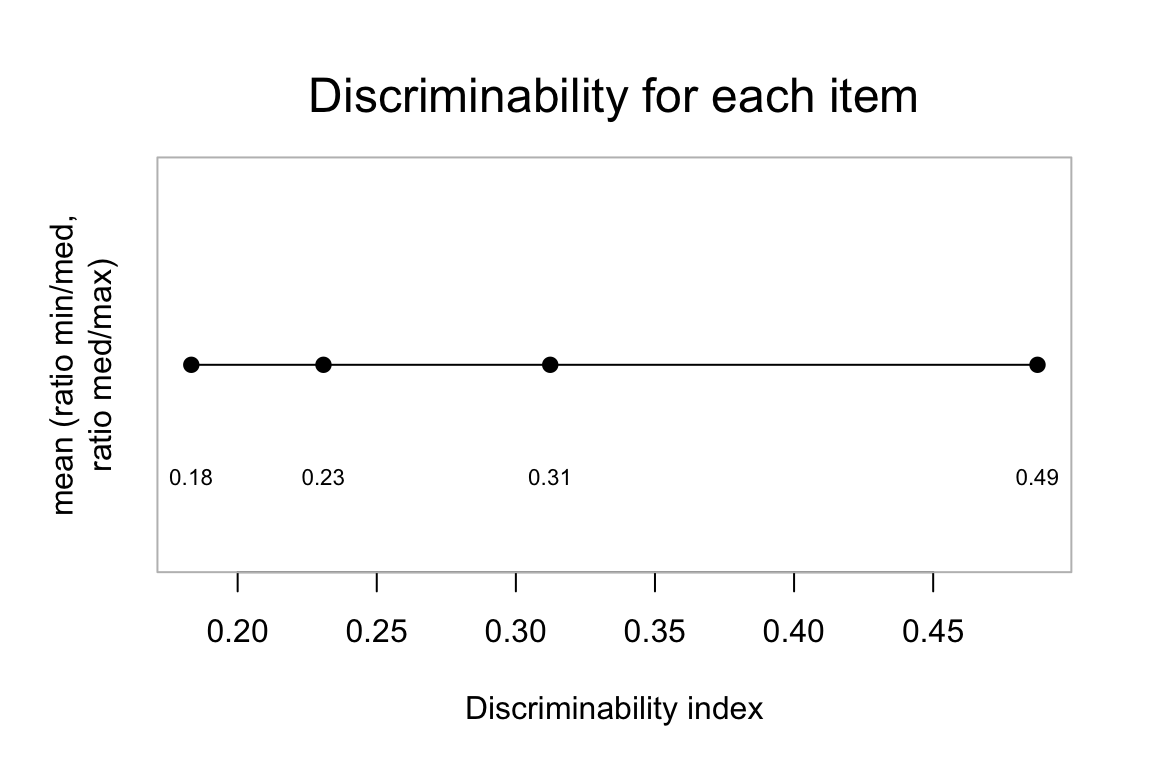
\includegraphics[width=\maxwidth]{figure/showCompression-1} \caption[Show compression of item ratios]{Show compression of item ratios}\label{fig:showCompression}
\end{figure}


\end{knitrout}

\FloatBarrier
\section{Lmer model}

\begin{knitrout}
\definecolor{shadecolor}{rgb}{0.969, 0.969, 0.969}\color{fgcolor}\begin{kframe}
\begin{alltt}
\hlkwd{load}\hlstd{(}\hlstr{"data_processed.Rda"}\hlstd{)}
\end{alltt}
\end{kframe}
\end{knitrout}

\begin{knitrout}
\definecolor{shadecolor}{rgb}{0.969, 0.969, 0.969}\color{fgcolor}\begin{kframe}
\begin{alltt}
\hlstd{v5} \hlkwb{<-} \hlstd{lmerTest}\hlopt{::}\hlkwd{lmer}\hlstd{(}\hlkwc{data}\hlstd{=dd,}
\hlstd{RT_log} \hlopt{~}
\hlstd{c_Vag} \hlopt{+} \hlstd{c_Num} \hlopt{+} \hlstd{c_Qty} \hlopt{+} \hlstd{c_Ord} \hlopt{+}
\hlstd{c_Num}\hlopt{:}\hlstd{c_Vag}\hlopt{:}\hlstd{c_Qty} \hlopt{+}
\hlstd{item_mean_ratio} \hlopt{+}
\hlstd{s_Trl} \hlopt{+}
\hlstd{RTprev_log} \hlopt{+}
\hlstd{nchar_instr} \hlopt{+}
\hlstd{(}\hlnum{1}\hlopt{+}\hlstd{c_Vag} \hlopt{+} \hlstd{c_Num} \hlopt{+} \hlstd{c_Qty} \hlopt{+} \hlstd{c_Ord}\hlopt{|}\hlstd{Subject))}
\hlstd{v5b} \hlkwb{<-} \hlstd{lme4}\hlopt{::}\hlkwd{lmer}\hlstd{(}\hlkwc{data}\hlstd{=dd,}
\hlstd{RT_log} \hlopt{~}
\hlstd{c_Vag} \hlopt{+} \hlstd{c_Num} \hlopt{+} \hlstd{c_Qty} \hlopt{+} \hlstd{c_Ord} \hlopt{+}
\hlstd{c_Num}\hlopt{:}\hlstd{c_Vag}\hlopt{:}\hlstd{c_Qty} \hlopt{+}
\hlstd{item_mean_ratio} \hlopt{+}
\hlstd{s_Trl} \hlopt{+}
\hlstd{RTprev_log} \hlopt{+}
\hlstd{nchar_instr} \hlopt{+}
\hlstd{(}\hlnum{1}\hlopt{+}\hlstd{c_Vag} \hlopt{+} \hlstd{c_Num} \hlopt{+} \hlstd{c_Qty} \hlopt{+} \hlstd{c_Ord}\hlopt{|}\hlstd{Subject))}
\end{alltt}
\end{kframe}
\end{knitrout}

\begin{knitrout}
\definecolor{shadecolor}{rgb}{0.969, 0.969, 0.969}\color{fgcolor}\begin{kframe}
\begin{alltt}
\hlkwd{summary}\hlstd{(v5)}
\end{alltt}
\begin{verbatim}
## Linear mixed model fit by REML t-tests use Satterthwaite approximations
##   to degrees of freedom [lmerMod]
## Formula: RT_log ~ c_Vag + c_Num + c_Qty + c_Ord + c_Num:c_Vag:c_Qty +  
##     item_mean_ratio + s_Trl + RTprev_log + nchar_instr + (1 +  
##     c_Vag + c_Num + c_Qty + c_Ord | Subject)
##    Data: dd
## 
## REML criterion at convergence: 11474.8
## 
## Scaled residuals: 
##     Min      1Q  Median      3Q     Max 
## -4.5470 -0.6351 -0.0955  0.5372  5.0914 
## 
## Random effects:
##  Groups   Name        Variance Std.Dev. Corr                   
##  Subject  (Intercept) 0.153949 0.39236                         
##           c_Vag       0.001546 0.03932   0.69                  
##           c_Num       0.165314 0.40659  -0.67 -0.64            
##           c_Qty       0.008148 0.09027   0.16  0.26 -0.34      
##           c_Ord       0.001559 0.03949  -0.13  0.02 -0.39 -0.52
##  Residual             0.249734 0.49973                         
## Number of obs: 7677, groups:  Subject, 30
## 
## Fixed effects:
##                     Estimate Std. Error         df t value Pr(>|t|)    
## (Intercept)        6.400e+00  1.252e-01  2.600e+02  51.112  < 2e-16 ***
## c_Vag              6.094e-02  1.387e-02  3.300e+01   4.393 0.000112 ***
## c_Num             -4.336e-01  7.515e-02  2.900e+01  -5.770 2.97e-06 ***
## c_Qty             -6.907e-02  2.005e-02  2.900e+01  -3.445 0.001743 ** 
## c_Ord              1.796e-02  1.350e-02  5.100e+01   1.331 0.189164    
## item_mean_ratio    7.714e-01  4.927e-02  7.551e+03  15.658  < 2e-16 ***
## s_Trl             -1.070e-01  5.807e-03  7.558e+03 -18.421  < 2e-16 ***
## RTprev_log         6.047e-02  9.692e-03  7.594e+03   6.239 4.63e-10 ***
## nchar_instr        6.086e-03  1.944e-03  7.551e+03   3.131 0.001749 ** 
## c_Vag:c_Num:c_Qty  1.049e-01  4.607e-02  7.551e+03   2.278 0.022742 *  
## ---
## Signif. codes:  0 '***' 0.001 '**' 0.01 '*' 0.05 '.' 0.1 ' ' 1
## 
## Correlation of Fixed Effects:
##             (Intr) c_Vag  c_Num  c_Qty  c_Ord  itm_m_ s_Trl  RTprv_ nchr_n
## c_Vag        0.083                                                        
## c_Num       -0.360 -0.337                                                 
## c_Qty        0.067  0.117 -0.278                                          
## c_Ord       -0.051  0.007 -0.206 -0.228                                   
## item_men_rt -0.257 -0.004  0.001  0.000 -0.001                            
## s_Trl       -0.104  0.003 -0.001 -0.002  0.006 -0.017                     
## RTprev_log  -0.587  0.006 -0.004 -0.003  0.019 -0.015  0.185              
## nchar_instr -0.505  0.237 -0.034  0.018  0.000 -0.017  0.000  0.006       
## c_Vg:c_N:_Q  0.070 -0.033  0.005 -0.003  0.000  0.002 -0.001 -0.002 -0.138
\end{verbatim}
\end{kframe}
\end{knitrout}

\begin{kframe}
\begin{alltt}
\hlkwd{print}\hlstd{(}\hlkwd{xtable}\hlstd{(}\hlkwd{coef}\hlstd{(}\hlkwd{summary}\hlstd{(v5b))))}
\end{alltt}
\end{kframe}% latex table generated in R 3.3.1 by xtable 1.8-2 package
% Wed Aug 10 22:41:39 2016
\begin{table}[ht]
\centering
\begin{tabular}{rrrr}
  \hline
 & Estimate & Std. Error & t value \\ 
  \hline
(Intercept) & 6.40 & 0.13 & 51.11 \\ 
  c\_Vag & 0.06 & 0.01 & 4.39 \\ 
  c\_Num & -0.43 & 0.08 & -5.77 \\ 
  c\_Qty & -0.07 & 0.02 & -3.45 \\ 
  c\_Ord & 0.02 & 0.01 & 1.33 \\ 
  item\_mean\_ratio & 0.77 & 0.05 & 15.66 \\ 
  s\_Trl & -0.11 & 0.01 & -18.42 \\ 
  RTprev\_log & 0.06 & 0.01 & 6.24 \\ 
  nchar\_instr & 0.01 & 0.00 & 3.13 \\ 
  c\_Vag:c\_Num:c\_Qty & 0.10 & 0.05 & 2.28 \\ 
   \hline
\end{tabular}
\end{table}


\begin{knitrout}
\definecolor{shadecolor}{rgb}{0.969, 0.969, 0.969}\color{fgcolor}\begin{kframe}
\begin{alltt}
\hlkwd{cat}\hlstd{(}\hlstr{"R^2"}\hlstd{)}
\end{alltt}
\begin{verbatim}
## R^2
\end{verbatim}
\begin{alltt}
\hlkwd{cor}\hlstd{(}\hlkwd{fitted}\hlstd{(v5), dd}\hlopt{$}\hlstd{RT_RecSqt)}\hlopt{^}\hlnum{2}
\end{alltt}
\begin{verbatim}
## [1] 0.5095834
\end{verbatim}
\end{kframe}
\end{knitrout}

\begin{knitrout}
\definecolor{shadecolor}{rgb}{0.969, 0.969, 0.969}\color{fgcolor}\begin{kframe}
\begin{alltt}
\hlkwd{par}\hlstd{(}\hlkwc{mfrow}\hlstd{=}\hlkwd{c}\hlstd{(}\hlnum{3}\hlstd{,}\hlnum{4}\hlstd{),} \hlkwc{family}\hlstd{=}\hlstr{'cmodern'}\hlstd{)}
\hlkwd{plotLMER.fnc}\hlstd{(v5)}
\end{alltt}
\begin{verbatim}
## effect size (range) for  c_Vag is  0.03470056 
## effect size (range) for  c_Num is  0.4073765 
## effect size (range) for  c_Qty is  0.09530422 
## effect size (range) for  c_Ord is  0.0179595 
## effect size (range) for  item_mean_ratio is  0.2346348 
## effect size (range) for  s_Trl is  0.369093 
## effect size (range) for  RTprev_log is  0.2759498 
## effect size (range) for  nchar_instr is  0.05477539
\end{verbatim}


{\ttfamily\noindent\bfseries\color{errorcolor}{\#\# Error in plot.new(): figure margins too large}}\end{kframe}
\end{knitrout}

Plot model coefficients and ci's

\begin{knitrout}
\definecolor{shadecolor}{rgb}{0.969, 0.969, 0.969}\color{fgcolor}\begin{kframe}
\begin{alltt}
\hlstd{e}\hlkwb{=}\hlkwd{data.frame}\hlstd{(}\hlkwc{coef}\hlstd{=}\hlkwd{summary}\hlstd{(v5)}\hlopt{$}\hlstd{coef[}\hlopt{-}\hlnum{1}\hlstd{,}\hlnum{1}\hlstd{])} \hlcom{# estimates, without intercept}
\hlstd{q}\hlkwb{=}\hlkwd{as.data.frame}\hlstd{(}\hlkwd{confint}\hlstd{(v5,} \hlkwc{method}\hlstd{=}\hlstr{'Wald'}\hlstd{)[}\hlnum{18}\hlopt{:}\hlnum{26}\hlstd{,}\hlnum{1}\hlopt{:}\hlnum{2}\hlstd{])}
\hlstd{eq}\hlkwb{=}\hlkwd{cbind}\hlstd{(e,q)}
\hlstd{y}\hlkwb{=}\hlstd{eq[}\hlkwd{rev}\hlstd{(}\hlkwd{rownames}\hlstd{(eq)),]}
\hlkwd{par}\hlstd{(}\hlkwc{mar}\hlstd{=}\hlkwd{c}\hlstd{(}\hlnum{4}\hlstd{,}\hlnum{10}\hlstd{,}\hlnum{1}\hlstd{,}\hlnum{1}\hlstd{))}
\hlkwd{plot}\hlstd{(}\hlkwc{y}\hlstd{=}\hlnum{1}\hlopt{:}\hlkwd{nrow}\hlstd{(y),} \hlkwc{x}\hlstd{=y}\hlopt{$}\hlstd{coef,} \hlkwc{xlim}\hlstd{=}\hlkwd{range}\hlstd{(y}\hlopt{$}\hlstr{"2.5 %"}\hlstd{, y}\hlopt{$}\hlstr{"97.5 %"}\hlstd{),} \hlkwc{type}\hlstd{=}\hlstr{'n'}\hlstd{,} \hlkwc{axes}\hlstd{=F,} \hlkwc{xlab}\hlstd{=}\hlstr{""}\hlstd{,} \hlkwc{ylab}\hlstd{=}\hlstr{""}\hlstd{)}
\hlkwd{segments}\hlstd{(}\hlkwc{y0}\hlstd{=}\hlnum{1}\hlopt{:}\hlkwd{nrow}\hlstd{(y),} \hlkwc{y1}\hlstd{=}\hlnum{1}\hlopt{:}\hlkwd{nrow}\hlstd{(y),} \hlkwc{x0}\hlstd{=y}\hlopt{$}\hlstr{"2.5 %"}\hlstd{,} \hlkwc{x1}\hlstd{=y}\hlopt{$}\hlstr{"97.5 %"}\hlstd{,} \hlkwc{lwd}\hlstd{=}\hlnum{.55}\hlstd{)}
\hlkwd{points}\hlstd{(}\hlkwc{y}\hlstd{=}\hlnum{1}\hlopt{:}\hlkwd{nrow}\hlstd{(y),} \hlkwc{x}\hlstd{=y}\hlopt{$}\hlstd{coef,} \hlkwc{pch}\hlstd{=}\hlnum{20}\hlstd{,} \hlkwc{cex}\hlstd{=}\hlnum{.75}\hlstd{)}
\hlkwd{abline}\hlstd{(}\hlkwc{v}\hlstd{=}\hlnum{0}\hlstd{,} \hlkwc{lty}\hlstd{=}\hlnum{3}\hlstd{,} \hlkwc{col}\hlstd{=}\hlstr{'grey'}\hlstd{)}
\hlkwd{axis}\hlstd{(}\hlnum{2}\hlstd{,} \hlkwc{labels}\hlstd{=}\hlkwd{row.names}\hlstd{(y),} \hlkwc{at}\hlstd{=}\hlnum{1}\hlopt{:}\hlkwd{nrow}\hlstd{(y),} \hlkwc{las}\hlstd{=}\hlnum{1}\hlstd{)}
\hlkwd{axis}\hlstd{(}\hlnum{1}\hlstd{,} \hlkwc{las}\hlstd{=}\hlnum{1}\hlstd{)}
\hlkwd{mtext}\hlstd{(}\hlstr{"estimate"}\hlstd{,} \hlkwc{side}\hlstd{=}\hlnum{1}\hlstd{,} \hlkwc{line}\hlstd{=}\hlnum{2.5}\hlstd{,} \hlkwc{cex.lab}\hlstd{=}\hlnum{1}\hlstd{,} \hlkwc{las}\hlstd{=}\hlnum{1}\hlstd{)}
\hlkwd{box}\hlstd{(}\hlkwc{col}\hlstd{=}\hlstr{'grey'}\hlstd{)}
\end{alltt}
\end{kframe}\begin{figure}
\includegraphics[width=\maxwidth]{figure/v54-1} \caption[Estimates plot]{Estimates plot}\label{fig:v54}
\end{figure}


\end{knitrout}
    
Model criticism baayen plots
    
\begin{knitrout}
\definecolor{shadecolor}{rgb}{0.969, 0.969, 0.969}\color{fgcolor}\begin{kframe}
\begin{alltt}
\hlcom{# Baayen 4-plot model criticism}
\hlkwd{par}\hlstd{(}\hlkwc{mfrow}\hlstd{=}\hlkwd{c}\hlstd{(}\hlnum{1}\hlstd{,}\hlnum{4}\hlstd{),} \hlkwc{pty}\hlstd{=}\hlstr{'s'}\hlstd{)}
\hlcom{# create scaled residuals}
\hlstd{dd}\hlopt{$}\hlstd{rstand} \hlkwb{=} \hlkwd{as.vector}\hlstd{(}\hlkwd{scale}\hlstd{(}\hlkwd{resid}\hlstd{(v5)))}
\hlcom{# plot scaled residuals density}
\hlkwd{plot}\hlstd{(}\hlkwd{density}\hlstd{(dd}\hlopt{$}\hlstd{rstand))}
\hlcom{# plot sample quantiles versus theoretical quantiles}
\hlkwd{qqnorm}\hlstd{(dd}\hlopt{$}\hlstd{rstand,} \hlkwc{cex}\hlstd{=}\hlnum{.5}\hlstd{)}
\hlkwd{qqline}\hlstd{(dd}\hlopt{$}\hlstd{rstand)}
\hlcom{# plot standardised residuals versus fitted values}
\hlkwd{plot}\hlstd{(dd}\hlopt{$}\hlstd{rstand} \hlopt{~} \hlkwd{fitted}\hlstd{(v5),} \hlkwc{pch}\hlstd{=}\hlstr{'.'}\hlstd{)}
\hlcom{# absolute standardised residuals greater than 2.5 are candidates for being outliers, the abline identifies them on the plot}
\hlkwd{abline}\hlstd{(}\hlkwc{h}\hlstd{=}\hlkwd{c}\hlstd{(}\hlopt{-}\hlnum{2.5}\hlstd{,}\hlnum{2.5}\hlstd{))}
\end{alltt}
\end{kframe}\begin{figure}
\includegraphics[width=\maxwidth]{figure/baayenPLots99-1} \caption[caption]{caption}\label{fig:baayenPLots99}
\end{figure}


\end{knitrout}

\end{document}
